\section{Challenges and Related Work}
\label{sec:ch8::challenges}


This section describes the major challenges for
hosting data-intensive applications on the cloud.

\subsection{Cost-Effective Cloud Configurations}

IaaS provides a wide range of resources configurations.
It is generally considered challenging to choose
the most cost-effective configurations.
In real-world application, trial-and-error is a common approach.
For example, a common workflow for Elastic MapReduce (i.e., Hadoop) in AWS
is for users to try out a handful of different configurations
as they develop an effective solution, which is then used for production.
A couple of times a year this process is repeated to re-optimizes
the configuration for the expanding dataset.

Choosing cost-effective configurations is time consuming and prone to
errors (suboptimal solutions in terms of cost and performance).
To facilitate this selection process, we need to
characterize applications and resources.
We also need to understand application performance and behavior
at different scales of data sizes.
None of these problems is straight forward.

\subsubsection*{Characterizing applications and resources}
Application performance is affected by
resource types, input workloads and
software configurations~\cite{Alipourfard2017}.
For example, task parallelism is a major factor to
performance of MapReduce programs~\cite{kc2015dynamically}.

\subsubsection*{Exhaustive exploration is not feasible}
Since the configuration space is very large, exhaustive search to
find the cost-effective configurations is not a feasible approach.
To reduce the cost of exploring such a large space,
performance \emph{extrapolation} is one way to reduce the cost.
Based on a relatively smaller training dataset,
we can predict application performance with different configurations or 
different data sizes~\cite{Hsu2016}.
We can also conduct iterative search while reducing the number of configurations
required to evaluate~\cite{Alipourfard2017}.


\subsection{Persistent Storage is Expensive or Insufficient}

Cloud computing is beneficial for both
periodical or dynamic changing workloads.
Infrastructure-as-a-Service allows ones to provision resources dynamically
to fit workload demands.
The cost of hosting applications is proportional to the period of
resources being provisioned.
Hosting data-intensive applications on the cloud requires handling
large-scale dataset.
The large storage resource incurs high costs, especially for
long term usages on the cloud.

Amazon Web Service offers several storage classes and charges them
at different prices, as listed in \mytable~\ref{tab:storage-costs}.
We consider two cases for storing data on AWS.
First, EFS acts both offline and online storage.
Second S3 is the offline storage and
EBS is provisioned while applications are running.
We conduct a cost analysis to compare the cost of these two choices
under different usage hours per day.
The target cluster size is 100 machines with data size is 100 TB.
\myfigure~\ref{fig:cost_analysis} shows that storage incurs very high
at-rest cost, \$30,000 dollars for 100 TB data on EFS.

To make data-intensive applications feasible on the cloud,
we need to choose affordable storage options and
ensure sustainable periodic execution.
This requires deep understandings about workload patterns and storage performance.
Without proper capacity planning, users are not willing to migrate
data-intensive applications to the cloud.

\begin{figure}
    \centering
    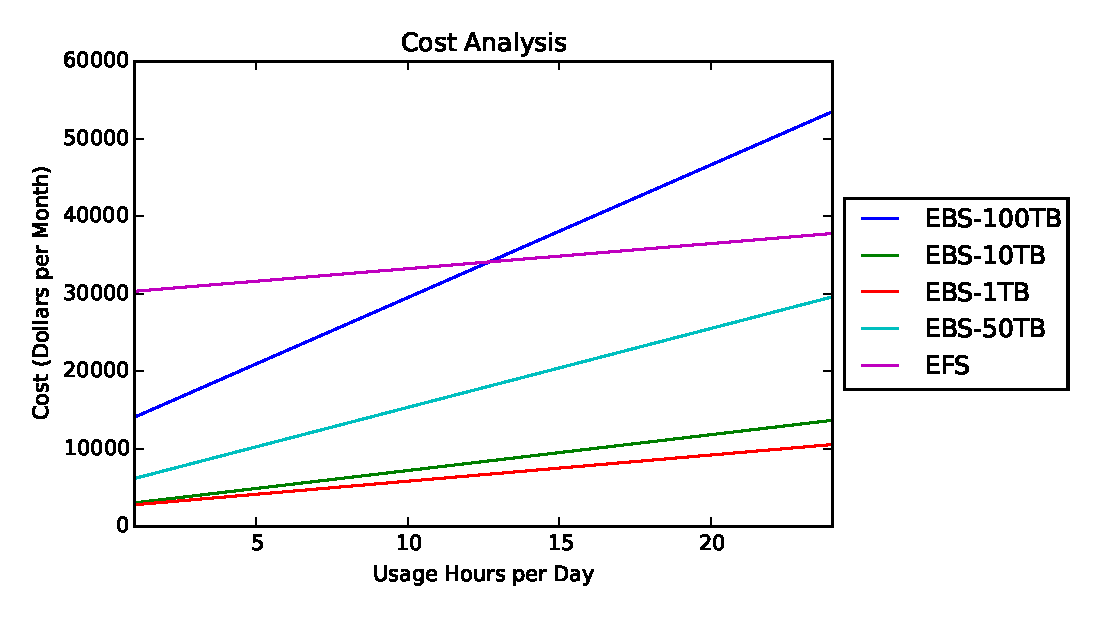
\includegraphics[width=0.9\textwidth]{Chapter-8/figures/cost_analysis.eps}
    \caption{Cost analysis of cloud storage options}
    \label{fig:cost_analysis}
\end{figure}


\subsection{Inefficient Job Scheduling for Cloud Storage}
Most large-scale data processing systems such as Hadoop, Spark and HPCC
are designed for commodity machines.
In such a \emph{reference model}, a machine serves
both compute and storage function
as described in Section~\ref{tab:model_comparison}.
These systems scale well because the compute and I/O ratio remains
almost constant as the number of machines increases.
However, when hosting data-intensive computing on the cloud, the model might not
be the most cost-effective architecture.
The \emph{remote storage} or \emph{cloud storage} model can be a better
storage architecture under the periodical workload and with large dataset.

Job scheduling in batch processing systems, e.g., Hadoop and Spark,
incorporates data locality for maximizing system throughput.
This approach greatly reduces the cost of data transmission over network.
Many job scheduling policies are not applicable to
the \emph{remote storage} or \emph{cloud storage} model because
data locality no longer exists.
In addition, I/O and network resources are scarce.
Without proper resource allocation, they lead to the performance bottleneck.
Therefore, we need a new scheduling method for optimizing system performance
for he \emph{remote storage} or \emph{cloud storage} model.